\chapter{Routing}
\label{chap:routing}

\section{Broadcast Routing mit Flooding}

Ein einfacher Weg, um eine Nachricht von einem Teilnehmer aus an alle anderen des Netzwerks zu senden, ist Flooding. Der Knoten, der senden möchte, sendet die Nachricht an alle seine Nachbarn. Diese leiten die Nachricht an alle Nachbarn weiter, ausser dem Knoten, von dem sie die Nachricht erhalten haben.
Das Problem dabei ist, dass dieser Algorithmus so nie enden würde (ausgenommen es gibt keine Zyklen im Netz).

Ein Lösungsansatz ist die Einführung eines numerischen \textbf{Hop Counters}, der auf den Nachrichten geführt wird. Bei der Weiterleitung auf einen Noten wird der Hop Counter immer um eins verringert. Ist der Counter bei Null angelangt, wird die Nachricht nicht mehr weitergeleitet, sondern verworfen.
Um sicher zu sein, dass alle Knoten des Netzes erreicht werden, wird der Hop Counter initialisiert mit dem Durchmesser (längste Distanz zwischen zwei Knoten) des Netzes.

Ein andere Möglichkeit, unendliche Broadcasts zu verhindern, ist mittels \textbf{Sequenznummern}. Wenn der Quellknoten die Nachrichten erstellt, wird jeder Nachricht eine eindeutige Sequenznummer zugewiesen. Jeder Knoten führt bei sich eine Tabelle, in der gespeichert wird, welche Sequenznummern von welchen Ursprungsknoten bereits erhalten wurden. Falls bereits ein Eintrag existiert, wird die Nachricht verworfen, andernfalls wird sie in die Tabelle eingetragen und anschliessend weitergeleitet an alle Nachbarn. 
Problematisch kann bei dieser Variante der Speicherplatzbedarf auf den Knoten werden, um sich alle Nachrichten aller Knoten zu merken.

Da die Sequenznummern immer hochgezählt werden, kann pro Knoten auch nur die jeweils höchste Nummer gespeichert werden. Man nimmt dabei an, dass die Broadcast Nachrichten grösstenteils mit aufsteigender Sequenznummer eintreffen.


Wegen der tieferen Message Komplexität (Tabelle \ref{tab:diff_routing}) wird normalerweise die Sequenznummer Variante der Hop Counter Methode vorgezogen. Nur bei Netzen resp. Graphen mit sehr geringem Durchmesser würde die Hop Counter Variante Vorteile bieten. 


\section{Unicast Routing mit Distance Vector}
Um in einem Netzwerk die kürzesten Pfade zwischen den verschiedenen Knoten zu finden, kann das Distance Vector Protokoll verwendet werden. Distance Vector kann mit verschienden Algorithmen realisiert werden. Hier wird die Variante basierend auf dem Algorithmus von Bellmann und Ford \cite{wiki:bellmannFord} beschrieben.

Es wird angenommen, dass alle Kanten im Graphen ein positives Gewicht haben.
Das Ziel ist, dass jeder Knoten weis, an welchen Knoten er ein eingegangenes Paket weiterleiten muss, damit es über den kürzesten Weg (geringstes Gewicht) zum Zielknoten kommt.
Dafür wird auf jedem Knoten eine Liste geführt, welche das Gesamtgewicht des Pfades zu jedem anderen Knoten enthält.

In einem Graphen mit vier Knoten A, B, C und D könnte die Liste auf Knoten A zum Beispiel so aussehen, wenn der Algorithmus fertig gelaufen ist:

\begin{figure}[ht]
	\centering
		\begin{minipage}[b]{0.45\linewidth}
			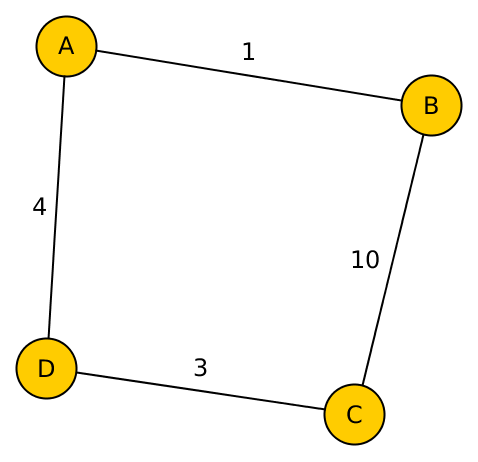
\includegraphics[width=0.6\textwidth]{bilder/distance_vector_example.png}
			\caption{Beispielgraph für Distance Vector}
		\end{minipage}
	\quad
		\begin{minipage}[b]{0.45\linewidth}
			\begin{center}
			\begin{tabular}{ |c|c|c| }
		 	\hline
		 	Ziel & Gewicht & weiter via  \\ 
		 	\hline
		 	A    & -       & -  \\ 
		 	B    & 1       & B  \\ 
		 	C    & 7       & D  \\ 
		 	D    & 4       & D  \\ 
		 	\hline
			\end{tabular}
			\end{center}
		\caption{Distance Vector auf Knoten A}
		\end{minipage}
\end{figure}



Die Einträge für die direkten Nachbarn können sofort erstellt werden. Die Gewichte für die anderen Knoten werden mit ''Infinity'' initialisiert.
Nun werden die Distance Vector Vector Informationen wird rundenbasiert aufgebaut.

In jeder Runde sendet jeder Knoten seine Distance Vector Information an alle direkten Nachbarn.
Sobald ein Knoten eine Distance Vector Nachricht erhalten hat, wird diese ausgewertet. Wenn eine kürzere Route gefunden wurde, wird der entsprechende interne Distance Vector Enitrag aktualisiert.

Um die Distance Vector Tabelle aufzubauen, muss jeder Knoten x $O(d_xn)$ Messages pro Runde verarbeiten ($d_x$ ist Anzahl Kanten des Knoten x). Im gesamten Netzwerk ergibt das $O(nm)$ Messages pro Runde. Der Algorithmus braucht so viele Runden, wie der Durchmesser D des Graphen ist. Somit ergibt sich eine Message Komplexität von $O(Dnm)$ \cite{goodrich2006algorithm}.

Das Routing Infomation Protocol (RIP) \cite{hedrick1988routing} verwendet den Distance Vector Algorithmus.


\section{Unicast Routing mit Link-State}
Ein anderer Algorithmus für Unicast Routing ist Link-State. Die Idee ist, dass in einer ersten Phase alle Knoten die Gewichte ihrer angrenzenden Kanten via Broadcast mit Sequenznummern im Neztwerk bekanntgeben. Danach ist auf jedem Knoten der 'Link-State' aller Knoten gespeichert und mittels dem Algorithmus von Dijkstra werden lokal die kürzesten Wege zu jedem Knoten berechnet und der jeweils erste Knoten im Pfad dahin wird gespeichert.

Das Routing Protocol OSPF \cite{moy1998rfc} ist ein bekanntes Beispiel für Link-State Routing.

Die lokale Berechung mittels einer Standard Implementation von Dijkstra läuft mit Zeitkomplexität $O(m\log{}n)$ \cite{wiki:dijkstra}. Der Speicherverbrauch auf den Knoten ist jeweils $O(n)$.

\newpage

\section{Vergleich von Broadcast und Unicast Algorithmen}

Folgende Tabelle vergleicht die vier beschriebenen Routing Algorithmen bezüglich folgender Kennwerte:
\begin{itemize}
	\item Messages: 		Anzahl Messages, die versendet werden
    \item Lokaler Speicher: Speicher, der auf jedem Knoten benötigt wird
    \item Lokale Zeit: 		Laufzeitverhalten auf den Knoten für die Weiterleitung einer Meldung
    \item Routing Zeit: 	Laufzeitverhalten für die Wegfindung einer Message
\end{itemize}
Der lokale Berechnungsaufwand, der auf den Knoten für den Aufbau von Datenstrukturen benötigt wird, wird hier nicht berücksichtigt. 

\begin{table}[H]
	\centering
		\begin{tabular}{p{0.2\textwidth} p{0.15\textwidth} p{0.15\textwidth} 		   p{0.15\textwidth}       p{0.2\textwidth}} \toprule
            \textbf{Algorithmus} & \textbf{Messages} 	& \textbf{Lokler Speicher} & \textbf{Lokle Zeit}  & \textbf{Routing Zeit} \\ \midrule
			Flooding Hop Counter & $O(1)$      			& $O(1)$ 				   & $O(d)$ 			  & $O((d_{max}-1)^{D})$  \\ \midrule
			Flooding Sequenz Nr. & $O(1)$      			& $O(n)$ 				   & $O(d)$ 			  & $O(m)$  			  \\ \midrule
			Distance Vector		 & $O(Dnm)$    			& $O(n)$ 				   & $O(1)$ 			  & $O(p)$  \\ \midrule
			Link-State			 & $O(m^{2})$  			& $O(n)$ 				   & $O(1)$ 			  & $O(p)$  \\ \midrule
		\end{tabular}
	\caption{Vergleich der asymptotischen Komplexität von statischen Routing Algorithmen \cite{goodrich2006algorithm}}
	\label{tab:diff_routing}
\end{table}

\begin{itemize}
	\item n: Anzahl Knoten im Netz
	\item m: Anzahl Kanten im Netz
    \item d: Maximaler Grad (max. Anzahl Kanten eines Knoten)
    \item D: Durchmesser des Netzwerks
    \item p: Anzahl Knoten des kürzesten Pfades
\end{itemize}
